%!TEX root = ../dokumentation.tex


\chapter{Implementation}\label{cha:Implementation}

Based on the previous introduction to the concept of the application, this chapter describes the implementation of the application in detail.

\section{Lexer}\label{sec:ImplementationLexer}

As mentioned in chapter \ref{sec:ConceptLexer} the implementation of the lexer consists of the definition of tokens in form of regular expression. The following paragraph presents defined tokens and their regular expressions.

In order to build the lexer, the function $lex.lex()$ is used. After the lexer has been created, the function $lex.token()$ returns matched tokens. The function $lex.token()$ is called until it returns a token of the type None that marks the end of the input stream. 

\subsection{Token}\label{sec:ImplementationLexerToken}

Tokens are given names that indicate what they represent. All tokens that have been defined are combined to a token list.   A tokens list is always required when writing a lexer using \ac{PLY} \cite{PLY}. The list of tokens is also used by the parser to identify terminal symbols \cite{PLY}. Listing \ref{lst:Lexer_tokens} shows the tokens list of the implemented lexer. \\

\begin{lstlisting}[language=Python,basicstyle=\scriptsize	,caption= Lexer tokens,label= lst:Lexer_tokens]
# List of token names
tokens = (
    'LGRAMMAR_EXPRESSION',
    'LTOKEN_EXPRESSION',
    'LSTRICT_EXPRESSION',
    'LMACRO_EXPRESSION',
    'NT_SYMBOL',
    'COMMENT',
    'OPEN_PARENTHESIS',
    'CLOSE_PARENTHESIS',
    'OPEN_SQUARE_BRACKET',
    'CLOSE_SQUARE_BRACKET',
    'ALTERNATIVE_SYMBOL',
    'REPETITION_SYMBOL',
    'T_SYMBOL'
)
\end{lstlisting}

\subsection{Regular expression}\label{sec:ImplementationLexerRegularExpression}

Tokens are specified by regular expressions. Regular expressions can be defined in a function. The name of the function is the name of one token in the tokens list with the prefix t\textunderscore . Inside a function it is possible to modify the value of the generated LexToken object and then return it. If not modified, the value of the object is not modified and remains the actual text that has been matched. The regular expression is specified as a string in the beginning of a function. An extract of all functions can be seen in listing \ref{lst:Lexer_regex}. The function for the token $COMMENT$ consists of the comments regular expression that has already been described in chapter \ref{sec:ConceptLexer} and returns the LexToken object unmodified. The functions of $OPEN\textunderscore SQUARE\textunderscore BRACKET$, $NT\textunderscore SYMBOL$ and $T\textunderscore SYMBOL$ (and the other tokens in the tokens list) are implemented similar to $COMMENT$. However, the function of $LGRAMMAR\textunderscore EXPRESSION$ and the functions of the other expressions modify the value of the LexToken object. Instead of the value being the actual text matched, the last three characters are removed. The Python method $rstrip()$ removes all white spaced from the value. Thus, the function returns a LexToken object with the value of the text belonging to the nonterminal symbol that the expression represents. The rule symbol is removed because the rule type is already present in the token type. \\

\begin{lstlisting}[language=Python,basicstyle=\scriptsize	,caption= Lexer regular expressions,label= lst:Lexer_regex]
def t_COMMENT(self, t):
    r'^%.*$'
    return t

def t_OPEN_SQUARE_BRACKET(self, t):
     r'\['
     return t

def t_LGRAMMAR_EXPRESSION(self, t):
     r'<\w+>[\s]*::='
     t.value = t.value[:-3]
     t.value = t.value.rstrip()
     return t

def t_NT_SYMBOL(self, t):
     r'<\w+>'
     return t

def t_T_SYMBOL(self, t):
     r'[$\'\\\.,a-zA-Z\_0-9\0-9-\-<>&@!:{}~?^+=/"!^^/@/+-/%;][a-zA-Z\_0-9\-/"!?/@/+-/*/%;\->&+=$\'\\\.,]*'
     return t
)
\end{lstlisting}

The function $t\textunderscore ignore$ is used for declaring characters that should be ignored in the input stream. In this project, white spaced and new lines are ignored (see chapter \ref{sec:ConceptLexer}.

The function $t\textunderscore error$ is called when an error occurs during lexing. The defined error function shown in listing \ref{lst:Lexer_error} prints the value of the illegal character and skips the character. \\

\begin{lstlisting}[language=Python,basicstyle=\scriptsize	,caption= Lexer error function,label= lst:Lexer_error]
def t_error(self, t):
    print("Illegal character '%s'" % t.value[0])
    t.lexer.skip(1)
)
\end{lstlisting}


%
%\subsubsection{Ignored symbols}
%It is possible to declare symbols that should be ignored. However, if a symbol is declared as ignored but is specially mentioned in another token, then if the sequence
%of characters represent that token, the ignored symbol is not ignored. In this project, tabs and white spaces are ignored as they do not have any special meaning other than providing clarity.
%Also, newlines are generally ignored because as can be seen in listing \ref{lst:Lexer_example_multiline} there are rules that cover multiple lines.
%
%\begin{lstlisting}[basicstyle=\scriptsize	,caption= Multi line production rule,label= lst:Lexer_example_multiline]
%<annotated_formula>    ::= <thf_annotated> | <tff_annotated> | <tcf_annotated> |
%                           <fof_annotated> | <cnf_annotated> | <tpi_annotated>
%\end{lstlisting}
%
%Apart from the ignored symbols, there are 13 defined tokens:
%
%\subsubsection{Expressions}
%
%Expressions can either be of the type grammar, token, strict or macro. It is defined as a nonterminal symbol followed by the production symbol itself (::=,:==,:::,...). The nonterminal symbol and the production are merged to a single token and are not identified as two tokens to avoid ambiguity while parsing. If not it would be difficult for the parer to determine whether the nonterminal symbol that describes the rule is the start of a new rule or does still belong to the previous rule because as mentioned rules can cover multiple lines.
%
%\textit{Regular expression of grammar expression:}  $<\backslash w+>[\backslash s]*::=$
%
%$\backslash w+$ matches any alphanumeric and underscore character that can occur more than one time.
%$[\backslash s]*$ matches an arbitrary amount of white spaces. $::=$ matches the symbol for grammar expression and can be substituted  by any other symbol for the other expressions.
%
%\subsubsection{Nonterminal symbol}
%
%A nonterminal symbol starts with \dq <\dq\; and ends with \dq >\dq. In between there is any arbitrary sequence of numbers, underscores and small or capital letters which can be represented by $\backslash w+$ in a regular expression.
%
%\textit{Regular expression of nonterminal symbol:}  $<\backslash w+>$
%
%\subsubsection{Terminal symbol}
%
%%\textit{Regular expression of grammar expression:}  $'[$\backslash '\backslash \backslash \backslash .,a-zA-Z\backslash \textunderscore 0-9\backslash 0-9-\backslash -<>&@!:{}~?^+=/"!^^/@/+-/%;][a-zA-Z\_0-9\-/"!?/@/+-/*/%;\->&+=$\'\\\.,]*'$
%
%\subsubsection{Comment}
%
%A comment is identified by the lexer as a start of a new line followed by a percentage sign followed by an arbitrary character and ends with a newline. Because the percentage sign is also part of the terminal symbols, it is necessary to check whether the percentage sign is in a newline because the terminal symbol is not because the percentage symbol when used as terminal symbol is embedded in square brackets.    
%
%\textit{Regular expression of comment:}  $\textasciicircum \%.*\textdollar $
%%$'^%.*\textdollar '$
%
%\subsubsection{Meta-Symbols}
%
%Meta-Symbols include open and close parentheses \dq( )\dq, open and close square brackets \dq[ ]\dq, asterisks \dq *\dq and vertical bars \dq |\dq.
%
%They are recognized by the symbol itself and have a greater meaning for the parser as they impact the to be build data structures. 


\section{Parser}\label{sec:ImplementationParser}
The parser takes the matched tokens from the lexer and constructs a grammar list (see chapter \ref{sec:ConceptParser}) based on a specified context free grammar. Each rule of the context free grammar is defined by a Python function. The docstrings of the functions contain a context free grammar specification of the rules. The function accepts one argument which is a list of grammar symbols. The function contains semantic actions initiated by the rule that are applied to the first element of the input argument.
An example for a defined function can be seen in listing \ref{lst:Parser_functionProductionslist}. The function defines the rule that has the nonterminal symbol $productions\textunderscore list$ on the left side. The docstring of the functions contains the specification of the rule and the code inside the function determines the actions that are taken once the function is called. If the input has the length 2, meaning the input list consists of two entries, a new $PRODUCTIONS\textunderscore LIST$ is created with $p[1]$ and is saved in $p[0]$. If the length of the input equals four, a $productions\textunderscore list$ already exists and is expanded by a new productions alternative. This is done by appending $p[3]$ to the existing list that is stored in $p[1]$. The result is again being stored in $p[0]$. \\

\begin{lstlisting}[language=Python,basicstyle=\scriptsize	,caption= Parser function of productions list,label= lst:Parser_functionProductionslist]
def p_productions_list(self, p):
		"""
    productions_list : production
                     | productions_list ALTERNATIVE_SYMBOL production
    """
    if len(p) == 2:
    	p[0] = PRODUCTIONS_LIST([p[1]])
    elif len(p) == 4:
        p[1].list.append(p[3])
        p[0] = p[1]
\end{lstlisting}

The function that is defined first in the Python file determines the start symbol to which the grammar should be reduced. The parser stops when no more input exists and the start symbol has been reached. The final value is p[0] from the start symbol. 

The full defined context free grammar is presented in the following section \ref{sec:ImplementationGrammar}.

\subsection{Defined grammar}\label{sec:ImplementationGrammar}
The grammar is formally specified $G = (N,\sum,P,S)$.

$N$ is the set of nonterminal symbols. The set includes grammar list, comment block, grammar expression, token expression, strict expression, macro expression, productions list, production, xor productions list, t symbol production and production element.

$\sum$ is the set of terminal symbols. Terminal symbols of the specified grammar are the tokens generated by the lexer (see \ref{sec:ImplementationLexerToken}).

$P$ is the set of production rules that is presented in the following. 

A grammar list implies a comment block, the four expressions or a grammar list followed by the expressions.

\begin{align*}
	grammar\;list\; \rightarrow\; &comment\;block
	     		\mid grammar\;expression  \\
			   &\mid token\;expression
                \mid strict\;expression\\
               &\mid macro\;expression \\
               &\mid grammar\;list\;\;\;grammar\;expression\\
               &\mid grammar\;list\;\;\;strict\;expression \\
               &\mid grammar\;list\;\;\;macro\;expression \\
               &\mid grammar\;list\;\;\;comment\;block               
\end{align*}

A comment block is either a comment or a comment block with a comment.

\begin{align*}
    comment\;block\; \rightarrow\; &\textbf{comment}
                \mid comment\;block\;\;\textbf{comment}
\end{align*}

The four expressions are the expression token followed by their productions list. Grammar expression has a special case without a productions list because the production rule $<null>::= $ of the \ac{TPTP} grammar has no production on the right side. 

\begin{align*}
	grammar\;expression\; \rightarrow\; &\textbf{l grammar expression}\;\;productions\;list \\ 
               &\mid \textbf{l grammar expression} 
\end{align*}
\begin{align*}        
	token\;expression\; \rightarrow\; &\textbf{l token expression} \;\;productions\;list \\ \\
	strict\;expression\; \rightarrow\; &\textbf{l strict expression} \;\;productions\;list \\ \\
	macro\;expression\; \rightarrow\; &\textbf{l macro expression} \;\;productions\;list 
\end{align*}

Productions list and xor productions list imply either a production or a productions list alternative symbol production.
\begin{align*}
        productions\;list\; \rightarrow\; &production \\
               &\mid productions\;list\;\;\textbf{alternative symbol} \;production \\ \\                  
        xor\;productions\;list\; \rightarrow\; &production \\
               &\mid xor\;productions\;list\;\;\textbf{alternative symbol}\;production
\end{align*}
T symbol production is either a t symbol or a t symbol/repetition symbol/ alternative symbol embedded in square brackets.

\begin{align*}
	t\;symbol\;production\; \rightarrow\; & \textbf{open square bracket \; t symbol} \\ &\textbf{close square bracket}\\
               &\mid \textbf{open square bracket \; repetition symbol} \\ &\textbf{close square bracket}\\
               &\mid \textbf{open square bracket \; alternative symbol } \\ &\textbf{close square bracket}\\
               &\mid \textbf{t symbol} 
\end{align*}

Production element can be replaced by a nt symbol or by a nt symbol in square brackets or nt symbol repetition. In the case of repetition or square brackets the production element is categorized as optional when in square brackets or as repetition when followed by the repetition symbol. The same applies to t symbol production. A production element can also only be square brackets only.

 

\begin{align*}
	production\;element\; \rightarrow\; & \textbf{open square bracket \; nt symbol} \\ 
			   &\textbf{close square bracket}\\
               &\mid \textbf{nt symbol \; repetition symbol} \\
               &\mid t\;symbol\;production\;\; \textbf{repetition symbol} \\
               &\mid \textbf{open square bracket \; close square bracket} \\
               &\mid \textbf{nt symbol} \\
               &\mid t\; symbol\; production 
\end{align*}

\begin{align*}
	production\; \rightarrow\; &production\; element
                \mid production\;\; production\; element \\
               &\mid \textbf{open parenthesis}\;\; xor\; \;productions\; list\;\; \\
               &\textbf{close parenthesis} \\
               &\mid \textbf{open parenthesis}\;\; production\;\; \textbf{close parenthesis} \\
               &\mid production \;\;\textbf{open parenthesis}\;\; production \\
               &\textbf{close parenthesis} \\
               &\mid production\;\; \textbf{open parenthesis} \;\;xor \;productions\; list\\
               &\textbf{close parenthesis} \\
               &\mid \textbf{open parenthesis} \;\;production \;\;\textbf{close parenthesis} \\
               &production \\
               &\mid \textbf{open parenthesis}\;\; xor\; productions\; list\\ 
               &\textbf{close parenthesis}\;\; production \\
               &\mid \textbf{open parenthesis}\;\; production\;\; \textbf{close parenthesis} \\
               &\textbf{repetition symbol}\\
               &\mid production\;\; \textbf{open parenthesis} \;\;production \\
               &\textbf{close parenthesis \; repetition symbol}
\end{align*}


The start symbol is not specifically mentioned because it is per convention the left element of the first rule.

\subsubsection{Example}
Listing \ref{lst:Parser_example_productionelement} shows the production rule of the nonterminal $<tfx tuple>$ as well as the tokens that have been generated by the lexer. Using this single production, the functionality of the parser should be exemplified. \\

\begin{lstlisting}[basicstyle=\scriptsize	,caption= Production element,label= lst:Parser_example_productionelement]
<tfx_tuple>            ::= [] | [<tff_arguments>]
is made of tokens:
l grammar expression open square bracket close square bracket alternative symbol open square bracket nt symbol close square bracket
\end{lstlisting}

The resulting output of the parser can be seen in figure \ref{fig:ImplementationParsing}. The tokens have been reduced to the start symbol grammar list and are displayed in a form of a tree. Internally, the grammar list is stored as a nested list.

\begin{figure}[H]
\begin{tikzpicture}[
  ->,>=stealth',
  level/.style={level distance=1.5cm,sibling distance=4cm},
  level 2/.style={sibling distance=6cm},
  level 3/.style={sibling distance=5cm},
  level 5/.style={level distance=2cm, sibling distance=4cm},
  level 6/.style={level distance=2cm, sibling distance=4cm}
]
\node {grammar list}
    child{ node  {grammar expression} 
    		child{ node {\textbf{l grammar expression}}}
            child{ node {productions list} 
                child{ node  {productions list}
                	child {node {production}
                		child {node {productions element}
                			child{node {\textbf{\shortstack{open square bracket \\ close square bracket}}}}}}} 
                child{ node  {\textbf{alternative symbol}}}
                child{ node  {production}
                	child {node {productions element}
                		child{node {\textbf{\shortstack{open square bracket \\ nt symbol \\ close square bracket }}}}}}
                				}}
   
; 
\end{tikzpicture}
\caption{Parsing example}
\label{fig:ImplementationParsing}
\end{figure}
                
\subsection{Building the parser}\label{sec:ImplementationRunParser}

To build the parser the \ac{PLY} function $yacc.yacc()$ is called that constructs a parser from a specified grammar. To run the generated parser $parse()$ must be called. 

The output of the parser if further modified to include a numbering of the rules and to handle square brackets correctly (see chapter \ref{sec:ConceptDisambiguation}).
Rules are numbered by assigning the position of a rule within the grammar list as its position. Comment blocks are skipped. \\
The disambiguation of square brackets replaces the $ProductionProperty$ $Optional$ by the terminal symbols open and closing square bracket for $GRAMMAR$ and $STRICT$ expressions.
By doing so, the productions in the productions list of a rule are iterated. If the production has the production property $Optional$ the production property is changed to $None$ and square brackets are inserted in the production. This is done for productions as well as production elements that have the production property $Optional$ inside a production.


\section{Graph Builder}\label{sec:ImplementationGraphBuilder}

The class $TPTPGraphBuilder$ that can be seen in figure \ref{fig:ImplementationGraphbuilderUML} has an instance of the TPTPParser that has been introduced in chapter \ref{sec:ImplementationParser}. With the output of the parser, a grammar list, the graph builder builds a nodes dictionary and a graph. This is done by calling the $run$ method that calls $init\textunderscore tree$ for building the graph.
The methods highlighted in blue are used for building a graph and are described in chapter \ref{sec:ImplementationGraphGeneration}. The graph builder is also responsible for reducing the \ac{TPTP} grammar, the methods used for that are highlighted in turquoise and introduced in chapter \ref{sec:ImplementationExtractReducedGrammar}. Moreover, with the graph builder, comments are assigned to rules and nodes. Belonging methods are highlighted in green and described in chapter \ref{sec:ImplementationMaintainingComments}.

\begin{figure}[H]
\centering
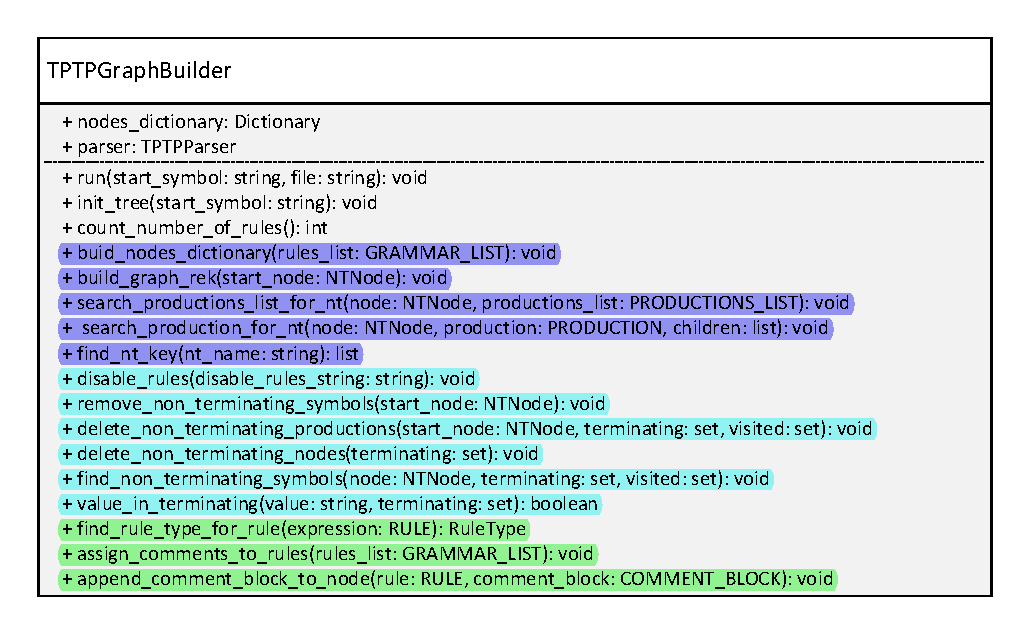
\includegraphics[width=1 \textwidth]{images/uml_graphbuilder.png}
\caption{Graphbuilder UML diagram}
\label{fig:ImplementationGraphbuilderUML}
\end{figure}                
                
\section{Graph generation}\label{sec:ImplementationGraphGeneration}

Before generating a graph, a node dictionary consisting of nodes is built. Figure \ref{fig:ImplementationNTNodeUML} shows the class NTNode that has already been introduced in chapter \ref{sec:ConceptGraphGeneration}. The class has three class methods:
$Add\textunderscore children$ adds a list of children to the existing nodes children list. $Extend\textunderscore comment\textunderscore block$ appends a comment block to the existing comment block of a node. The $str$ method is used for exporting the grammar.

\begin{figure}[H]
\centering
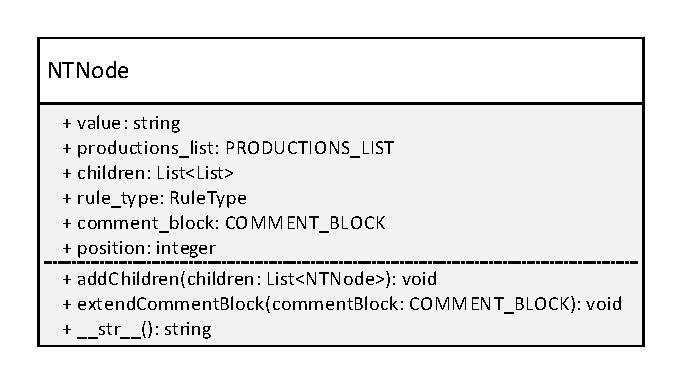
\includegraphics[width=1\textwidth]{images/uml_data_types_NTNode.pdf}
\caption{NTNode UML diagram}
\label{fig:ImplementationNTNodeUML}
\end{figure}

The rule type of a node is either grammar, token, strict or macro and is implemented as an enumeration that can be seen in figure \ref{fig:ImplementationRuleTypeUML}. 

\begin{figure}[H]
\centering
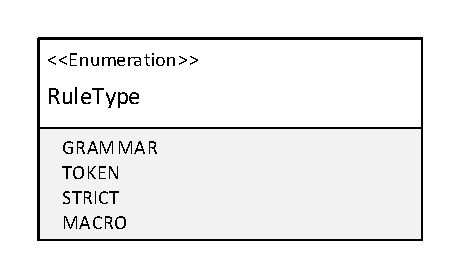
\includegraphics[width=.7\textwidth]{images/uml_data_types_rule_type.pdf}
\caption{RuleType UML diagram}
\label{fig:ImplementationRuleTypeUML}
\end{figure}

Algorithm \ref{alg:buildNodesDictionary} shows how the nodes dictionary is build. Iterating the rules list, a new dictionary item is created that consists of the node key rule name and rule type and the \textit{NTNode} as value. This is only the case if the rule is not a comment block. 
Listing \ref{lst:ImplementationMultipleSameRules} shows that multiple rules can exist that correspond to the same node.

\begin{lstlisting}[language=None, basicstyle=\scriptsize	,caption= Multiple rules with the same left-hand side of the rule,label= lst:ImplementationMultipleSameRules]
<defined_proposition>  :== <defined_predicate>
<defined_proposition>  :== $true | $false
<defined_predicate>    :== <atomic_defined_word>
<defined_predicate>    :== $distinct |
                           $less | $lesseq | $greater | $greatereq |
                           $is_int | $is_rat |
                           $box_P | $box_i | $box_int | $box |
                           $dia_P | $dia_i | $dia_int | $dia
\end{lstlisting}

If that would not have been considered, the second rule would create a new node and replace the existing on in the dictionary because their dictionary keys are the same. To not overwrite the node, the algorithm checks whether the key already exists in the dictionary. If the key already exists, the productions lists of the two rules are merged into one productions list that is appended to the node. 
After iterating, comments are assigned (see section \ref{sec:ImplementationMaintainingComments}).

\begin{algorithm}[H]
\caption{Graph Generation Algorithm: buildNodesDictionary}\label{alg:buildNodesDictionary}
\begin{algorithmic}[1] 
\Require rules\textunderscore list
\ForAll {rule in rules\textunderscore list} 
	\If {rule is not a comment block}
		\State rule\textunderscore type = this.find\textunderscore rule\textunderscore type\textunderscore for\textunderscore rule(rule)
		\State node\textunderscore key = Node\textunderscore Key(rule.name, rule\textunderscore type)
		\If {node\textunderscore key is not in this.nodes\textunderscore dictionary}
			\State node = NTNode(rule.name, rule.productions\textunderscore list, rule\textunderscore type, None, rule.position)
			\State this.nodes\textunderscore dictionary.update({node\textunderscore key:node})
		\Else
			\State node = this.nodes\textunderscore dictionary[node\textunderscore key]
			\State node.productions\textunderscore list.list.extend(rule.productions\textunderscore list.list)
		\EndIf
	\EndIf
\EndFor
\State Assign comments to rules
\end{algorithmic}
\end{algorithm}

To generate the graph of a given grammar three algorithms are needed that will be explained in the following.

The algorithm $buildGraphRek$ calls the function $searchProductionsListForNT$ that appends children of a node to the nodes list of children.
The algorithm is first called with the start symbol.
After the children of a node have been appended to the node, every child calls the algorithm resulting in appending their own children to their children's list.

\begin{algorithm}[H]
\caption{Graph Generation Algorithm: buildGraphRek}
\begin{algorithmic}[1] 
\Require node
%\ENSURE $y = x^n$
\State searchProductionsListForNT(node, node.productionsList)
\If {node has children}
	\ForAll {children}
		\State buildGraphRek(child)
	\EndFor
\EndIf
\end{algorithmic}
\end{algorithm}

The right side of a production rule is stored in a productions list.
For identifying the nonterminal or terminal symbols in the productions lists, a loop iterates all elements of the productions list.
Each element is a production and calls the function $searchProductionForNT$.
This function identifies the children of the given element who are then appended to the node.

\begin{algorithm}[H]
\caption{Algorithm for extracting productions from productions list: searchProductionsListForNT}
\begin{algorithmic}[1] 
\Require node, productionsList
\ForAll {elements in productionsList}
	\State children = new empty list
	\State searchProductionForNT(node, element in productionsList, children)
	\State append children to node
\EndFor
\end{algorithmic}
\end{algorithm}

The goal is to identify the nonterminal symbols.
Therefore, it is checked if the production is a nested production and if so, the same function is called again.
If the production is a XOR production list the function $searchProductionsListForNT$ is called to break down the productions list.
If the production element is a nonterminal symbol, the element is searched in the node dictionary to get the node where the element is on the left side.
This element is then appended to a list of children. It is possible that an element appears multiple times on the left side if it is presented by multiple expressions.
In this case each element is appended to the list of children.

\begin{algorithm}[H]
\caption{Algorithm for appending children to node: searchProductionForNT}
\begin{algorithmic}[1] 
\Require node, productionsElement, children
\ForAll {elements in productionsElementList}
	\If {element is  a production}
		\State {searchProductionForNT(node, element, children)}
	\ElsIf {element is a XOR productions list}
		\State {searchProductionsListForNT}
	\ElsIf {element is a nonterminal symbol}
		\State find element(s) in node dictionary
		\State append element(s) to children
	\EndIf
\EndFor
\end{algorithmic}
\end{algorithm}

\section{Maintaining comments}\label{sec:ImplementationMaintainingComments}

This section describes the implementation of associating comments with rules in order to maintain comments in a generated sub-syntax.
The implementation follows the concept outlined in section \ref{sec:ConceptMaintainingComments}.
Comments are associated after the grammar graph has been generated.
They are associated to the node, that represents the rule they belong to.
For that, the \textit{NTNode} class has a \textit{COMMENT\textunderscore BLOCK} attribute (see \textit{NTNode} UML diagram in figure \ref{fig:ImplementationNTNodeUML}).\\
Associating comments with nodes has the advantage, that when the grammar graph is reduced, only the comments associated with the rules that are part of the sub-syntax are maintained and can also be printed when outputting the sub-syntax.\\

\subsection{Splitting comment blocks}\label{sec:ImplementationMaintainingCommentsSplitByTop}

The flow chart in figure \ref{fig:ImplementationMaintainingCommentSplitByTopOfPage} shows how a comment block is split into multiple comment blocks separating it by top of page lines.\\
First the indexes of the top of page lines are collected in a list (using method of \textit{COMMENT\textunderscore BLOCK}).
After that, the \textit{comment\textunderscore block\textunderscore list}, which will contain the generated \textit{COMMENT\textunderscore BLOCK}s, is initialized.
If the list, storing top of page line indexes, is empty, the original comment block is added to the \textit{comment\textunderscore block\textunderscore list}, because the comment block does not need to be split into multiple comment blocks because no top of page line is present.
Then the \textit{comment\textunderscore block\textunderscore list} is returned.\\
If the list of top of page line indexes is not empty, the first top of page line index is retrieved from the top of page indexes list.
It is also checked whether the first top of page index is unequal zero.\\
If that is the case, the first top of page index is not the first line of the original comment block, and a comment block can be constructed from the line(s) before.
In this case the first comment block can be constructed from the comment lines of the original comment block from index zero to the first top of page index.
This comment block is added to the \textit{comment\textunderscore block\textunderscore list}.\\
Then the \textit{index} variable, which represents an index on the \textit{top\textunderscore of\textunderscore page\textunderscore indexes} list, is initialized.
The \textit{index} is used to access the corresponding element of the \textit{top\textunderscore of\textunderscore page\textunderscore indexes} list.\\
Then it is checked if top of page line that corresponds to the top of page line index is the last line of the original comment block.
In that case, no further comment block needs to be added to the \textit{comment\textunderscore block\textunderscore list} and the \textit{comment\textunderscore block\textunderscore list} is returned.\\
Otherwise the start index of the next comment block is computed as the current \textit{top\textunderscore of\textunderscore page\textunderscore index} incremented by one (line after the top of page line).
There are two cases that have to be considered when determining the end index of the comment block.
Either there is another top of page line, in this case the comment block ends before that, or the currently indexed top of page line was the last one, in that case the end index is the end of the original comment block.
Then the new commend block is constructed with the before determined \textit{start} and \textit{end}.
This comment block is added to the \textit{comment\textunderscore block\textunderscore list}.
If the \textit{index} is at the end of the \textit{top\textunderscore of\textunderscore page\textunderscore index} list, the \textit{comment\textunderscore block\textunderscore list} is returned. If not, the \textit{index} variable is incremented and the process is repeated with the next top of page index.

\begin{figure}[H]
\centering
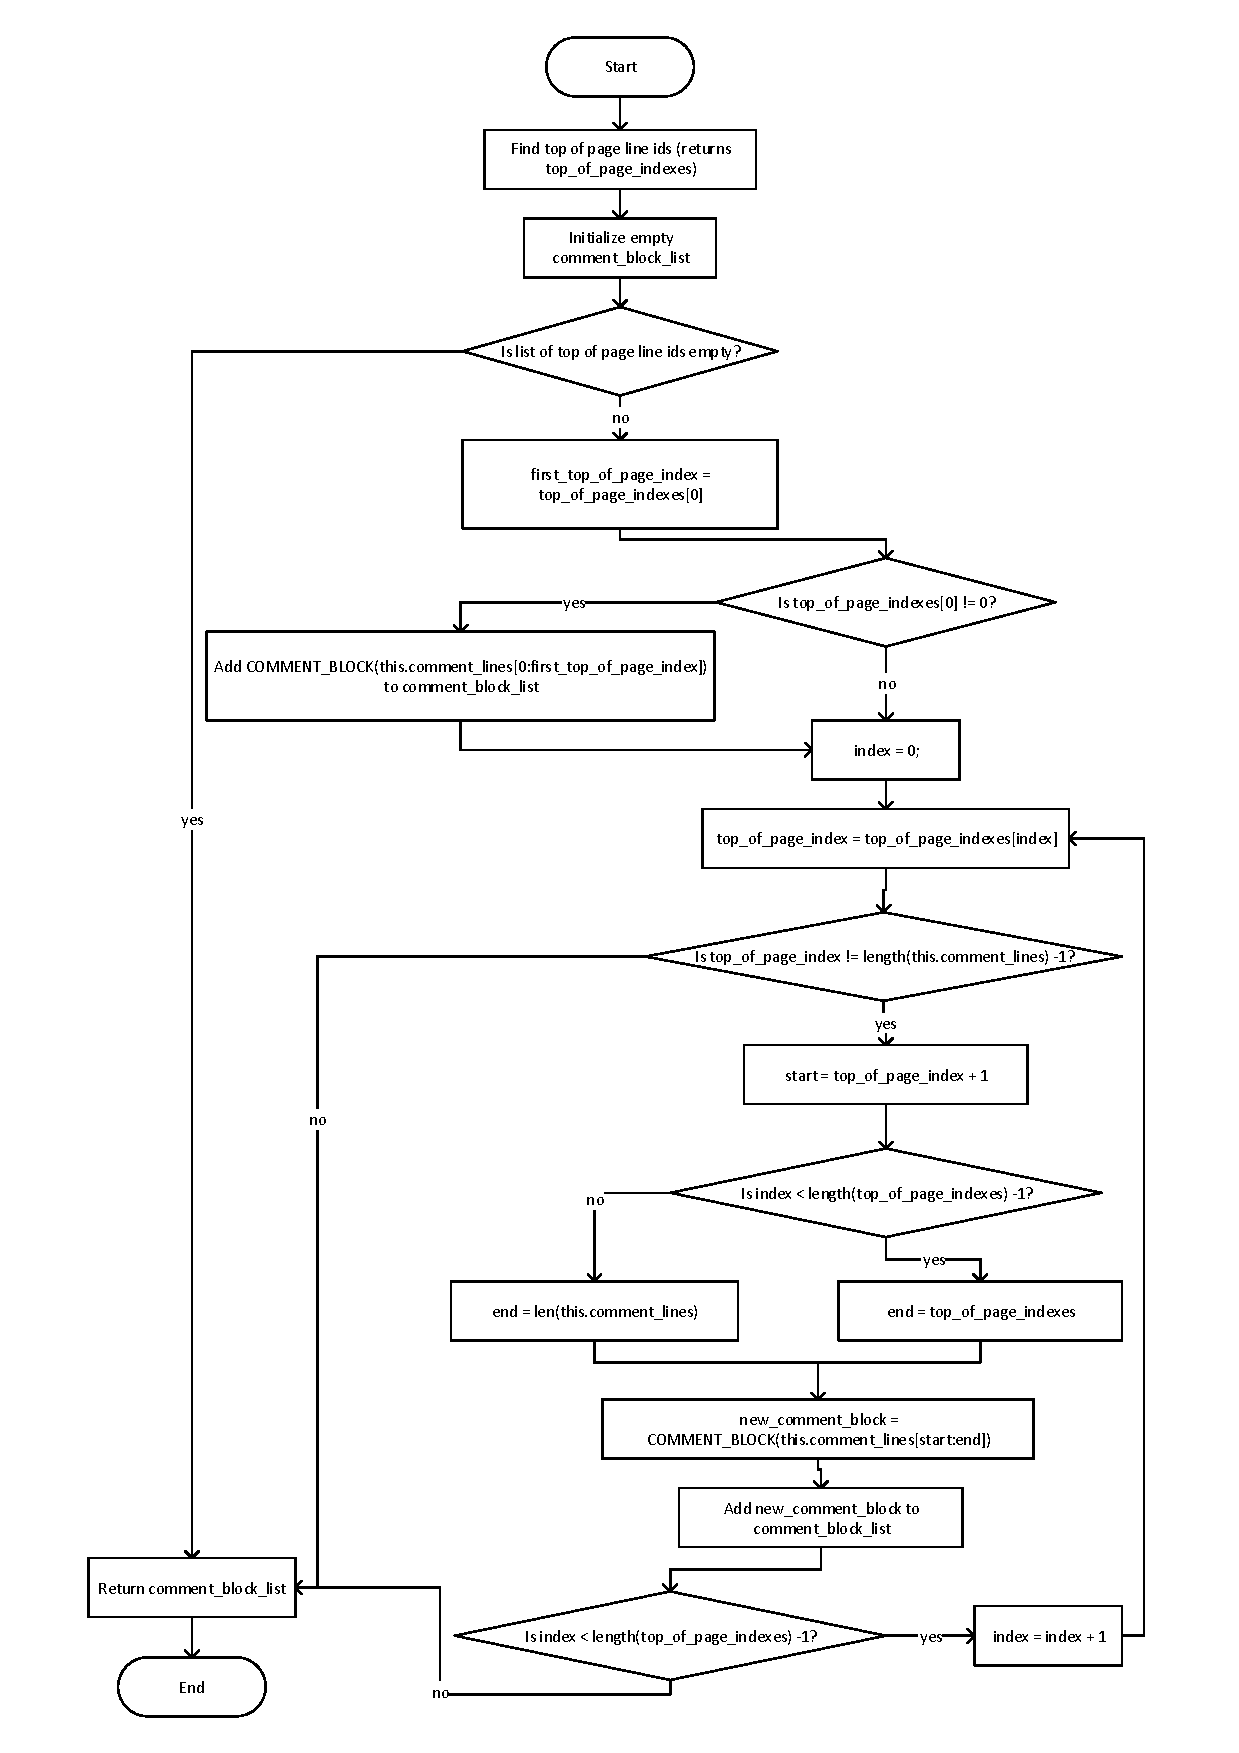
\includegraphics[width=1\textwidth]{images/Implementation_split_comment_by_top_of_page.pdf}
\caption{Split comment block by top of page line flow chart}
\label{fig:ImplementationMaintainingCommentSplitByTopOfPage}
\end{figure}

\subsection{Associating comments with grammar graph nodes}\label{sec:ImplementationMaintainingCommentsAssociateWithNodes}

Algorithm \ref{alg:assign_comments_to_rule} describes the procedure of matching comments to nodes. The algorithm follows the concept outlined in section \ref{sec:ConceptMaintainingComments} and is used within the \textit{TPTPGraphBuilder} after generating the grammar graph.\\
The input is the \textit{grammar\textunderscore list}, that the parser created from parsing the \ac{TPTP} syntax file.
The \textit{grammar\textunderscore list} contains rules and comment blocks in the order they appeared in the original \ac{TPTP} syntax file.
The \textit{grammar\textunderscore list} is iterated (line 1).\\
If the current element of the \textit{rules\textunderscore list} is a \textit{COMMENT\textunderscore BLOCK}, it is split by top of page lines (line 3).
The procedure of splitting a comment block by top of page lines is described in section \ref{sec:ImplementationMaintainingCommentsSplitByTop}.
It returns a list of comment block objects.\\
In the following if-clause it is checked, how many comment block objects are returned.\\
In the first case of one comment block, this comment block should be associated with the following rule by default. If that is not possible, because the comment block is at the end of the syntax file, it should be associated with the rule before.
In line 5 it is checked whether the comment block is not at the end of the syntax file. To associate the comment block with the following rule, the next rule (rule after the comment block) is obtained by indexing the next element of the \textit{rules\textunderscore list}.
Then, the comment block is appended to the node, specified by the rule, using the \textit{append\textunderscore comments\textunderscore to\textunderscore node} method. This method is described in the following subsection.\\
If the comment block is at the end of the syntax file, it has to be associated with the rule before.
This case is handled in the else branch (line 8).
The procedure of adding the comment block to the desired node is essentially the same as described before. The difference is that the previous rule is addressed (line 9).\\
If splitting the original comment block by top of page lines results in two comment blocks the first is associated with the rule before and the second with the rule after on condition that the original comment block was neither at the end nor the beginning of the syntax file (lines 14, 15, 21, 22).\\
If the original comment block was at the beginning of the syntax file, the first comment block is appended to the rule 
after too (lines 17, 18).\\
If the original comment block was at the end of the syntax file, the second comment block is associated with the rule before.\\
The case of two or more top of page lines does not occur in the \ac{TPTP} syntax version 7.3.0. and is not included in the pseudo-code.\\
This hypothetical case is handled by using the same procedure as in the case of two comment blocks but treating all comment blocks after the second comment block like the second. This means that all comment blocks from the second on would be associated with the rule after, except the case that the original comment block was at the end of the syntax file. In that case all comment blocks would be appended to the rule before.

The algorithm relies on the \textit{rules\textunderscore list} never having two or more comment blocks in a row (meaning they are always separated by at least one rule). This is ensured by the parser, because all consecutive comment lines in the syntax file are included into one comment block. Therefore consecutive comment block objects do not occur in the \textit{rules\textunderscore list}.

\begin{algorithm}[H]
\small
\caption{Assign comments to rules}
\begin{algorithmic}[1]
\algrenewcommand\algorithmicindent{0.7em}
\Require grammar\textunderscore list
\ForAll {index, expression in rules\textunderscore list.list}
	\If {expression is COMMENT\textunderscore BLOCK}
		\State {comment\textunderscore block\textunderscore list = expression.split\textunderscore comment\textunderscore block\textunderscore by\textunderscore top\textunderscore of\textunderscore page()}
		\If{length(comment\textunderscore block\textunderscore list) == 1}
			\If{index < length(rules\textunderscore list.list) - 1}
				\State {next\textunderscore rule = rules\textunderscore list.list[index + 1]}
				\State this.append\textunderscore comments\textunderscore to\textunderscore node(next\textunderscore rule, comment\textunderscore block\textunderscore list[0])
				\Else
					\State previous\textunderscore rule = rules\textunderscore list.list[index - 1]
					\State this.append\textunderscore comments\textunderscore to\textunderscore node(previous\textunderscore rule, comment\textunderscore block\textunderscore list[0])
			\EndIf
		\ElsIf {length(comment\textunderscore block\textunderscore list) == 2}
			\If{index != 0}
				\State previous\textunderscore rule = rules\textunderscore list.list[index - 1]
				\State this.append\textunderscore comments\textunderscore to\textunderscore node(previous\textunderscore rule, comment\textunderscore block\textunderscore list[0])
			\Else
				\State {next\textunderscore rule = rules\textunderscore list.list[index + 1]}
				\State this.append\textunderscore comments\textunderscore to\textunderscore node(next\textunderscore rule, comment\textunderscore block\textunderscore list[0])
			\EndIf
			\If{index < length(rules\textunderscore list.list) - 1)}
				\State {next\textunderscore rule = rules\textunderscore list.list[index + 1]}
				\State this.append\textunderscore comments\textunderscore to\textunderscore node(next\textunderscore rule, comment\textunderscore block\textunderscore list[1])
			\Else
				\State previous\textunderscore rule = rules\textunderscore list.list[index - 1]
				\State this.append\textunderscore comments\textunderscore to\textunderscore node(previous\textunderscore rule, comment\textunderscore block\textunderscore list[1])
			\EndIf
		\ElsIf{length(comment\textunderscore block\textunderscore list) > 2}
		\State \%excluded
		\EndIf
	\EndIf
\EndFor
\end{algorithmic}
\label{alg:assign_comments_to_rule}
\end{algorithm}

\subsubsection{Appending a comment block to a node}\label{sec:ImplementationMaintainingCommentBlockWithNodes}

In Algorithm \ref{alg:append_comment_to_node} it is described, how a comment block is appended to a node from the grammar graph, using information from the original rule created by the parser to address the node.\\
To associate the \textit{COMMENT\textunderscore BLOCK} with the node representing the rule, the node needs to be accessed.
It is more efficient to use the created \textit{nodes\textunderscore dictionary} to access the desired nodes than to traverse the grammar graph for each wanted node.\\
In the \textit{nodes\textunderscore dictionary}, the key for each node consists of the nonterminal symbol name and the \textit{RuleType} is stored(see section \ref{sec:ImplementationGraphGeneration}).\\
The rule type of the input rule is indicated by the type of the \textit{rule} object (see class diagram in figure \ref{fig:ImplementationRuleTypeUML}).
To index the node in the \textit{nodes\textunderscore dictionary} the \textit{RuleType} corresponding to the type of the rule object is needed.
The \textit{find\textunderscore rule\textunderscore type\textunderscore for\textunderscore rule} method determines and returns the \textit{RuleType} corresponding to the \textit{rule} object type.\\
Using the determined \textit{RuleType} and the nonterminal name, which is stored in the \textit{rule}, the key for the \textit{Nodes\textunderscore Dictionary} can be constructed (line 8).
Then, the node, to which the \textit{COMMENT\textunderscore BLOCK} should be added is addressed in the \textit{Nodes\textunderscore Dictionary} and the \textit{extend\textunderscore comment\textunderscore block} method of the node called, with the \textit{COMMENT\textunderscore BLOCK} as argument.
The \textit{extend\textunderscore comment\textunderscore block} method is described in algorithm \ref{alg:extend_comment_block}.
It appends the \textit{COMMENT\textunderscore BLOCK} to the \textit{COMMENT\textunderscore BLOCK} attribute of the node object.

\begin{algorithm}[H]
\small
\caption{Append comments to node}
\begin{algorithmic}[1]
\algrenewcommand\algorithmicindent{0.4em}
\Require rule, comment\textunderscore block
\State rule\textunderscore type = find\textunderscore rule\textunderscore type\textunderscore for\textunderscore rule(rule)
\State node\textunderscore key = Node\textunderscore Key(rule.name,rule\textunderscore type)
\State this.nodes\textunderscore dictionary[node\textunderscore key].extend\textunderscore comment\textunderscore block(comment\textunderscore block)
\end{algorithmic}
\label{alg:append_comment_to_node}
\end{algorithm}

\subsubsection{Extending a comment block of a node}\label{sec:ImplementationMaintainingExtendCommentBlock}

Algorithm \ref{alg:extend_comment_block} shows the procedure that is used in the \textit{extend\textunderscore comment\textunderscore block} method of the \textit{NTNode} class.
If no \textit{comment\textunderscore block} has not been associated with the node before, the input \textit{comment\textunderscore block} is associated with the node.
If the node has already have a \textit{comment\textunderscore block}, this \textit{comment\textunderscore block} is extended, with the comments lines from the input \textit{comment\textunderscore block}.\\
This procedure is needed because it is possible that multiple comment blocks, that have been generated on splitting comment blocks, have to be associated with the same node.

\begin{algorithm}[H]
\small
\caption{Extend node comment block}
\begin{algorithmic}[1]
\algrenewcommand\algorithmicindent{0.4em}
\Require comment\textunderscore block
\If {this.comment\textunderscore block is None}‚
	\State this.comment\textunderscore block = comment\textunderscore block
\Else
	\State this.comment\textunderscore block.extend(comment\textunderscore block.comment\textunderscore lines)
\EndIf
\end{algorithmic}
\label{alg:extend_comment_block}
\end{algorithm}

\section{Extraction of a sub-syntax}\label{sec:ImplementationExtractReducedGrammar}

The following sections describe the algorithms used for the extraction of a sub-syntax based on the concept outlined in section \ref{sec:ConceptExtractReducedGrammar}.

\subsection{Removal of blocked productions}

Algorithm \ref{alg:remove_blocked_productions} takes the text of the control file as an input argument (control file format description can be found in section \ref{sec:ConceptControlFile}) and removes the productions that should be blocked from the nodes.  
The control file string is split into a list of the lines (line 1).
The first line of the control file string, which describes the start symbol, is deleted from the list (line 2) because this information is not needed at this step.\\
Then the following lines are iterated:\\
For each line the content is split by the comma symbol, which produces a list of strings.
The first element of that list is the nonterminal symbol name of the symbol from which productions should be disabled.
The second element is the corresponding rule type symbol.
The nonterminal symbol name and the rule type, that is determined from the rules symbol (line 7), are stored in separate variables.
Then these elements are removed from the list and the remaining elements are converted to integers.
They are the indexes of the productions that should be removed.
The elements are ordered descending (line 10).
Ordering the indexes in that order has the advantage that, when the list of indexes is iterated to delete productions, the indexes of other productions that should be deleted are not changed by the deletion of productions before. To delete the productions from the specified node the node object has to be accessed.
This is done by addressing the node in the \textit{nodes\textunderscore dictionary} with its key consisting of the nonterminal symbol name and the rule type.
From the node, in a loop, the elements of the \textit{productions\textunderscore list} and the \textit{children} list corresponding to the indexes in the control file are deleted.

\begin{algorithm}[H]
\caption{Removing blocked productions}
\begin{algorithmic}[1] 
\Require control\textunderscore string
\State lines = control\textunderscore string.splitlines()
\State delete lines[0]
\ForAll {line in lines}
	\State data = line.splitBy(",")
	\State nonterminal\textunderscore name = data[0] 
	\State rule\textunderscore symbol = data[1]
	\State rule\textunderscore type = determineRuleType(rule\textunderscore symbol)
	\State delete data[0:2]
	\State data = parseInteger(data)
	\State data.sortReverse()
	\State node = this.nodes\textunderscore dictionary.get(Node\textunderscore Key(nonterminal\textunderscore name, rule\textunderscore type))
	\ForAll {index in data}
		\State delete node.productions\textunderscore list.list[index]
		\State delete node.children[index]
	\EndFor
\EndFor
\end{algorithmic}
\label{alg:remove_blocked_productions}
\end{algorithm}

\subsection{Determination of the remaining terminating symbols}

After the desired productions have been deleted from the grammar graph, the next step is to remove the nonterminating symbols from the grammar graph. Algorithm \ref{alg:remove_non_terminating_symbols} shows the procedure of how to remove nonterminating symbols.
First it has to be determined which symbols are terminating and which are nonterminating.

-one way: starting from terminal symbol, find nonterminal symbol that derives terminal symbol, then find nonterminal symbol that only produces terminating symbols
-graph data structure can only be traversed top down not bottom up.
-therefore start at start node, traverse graph, and find terminating symbols
-initialise visited set
-store known terminating symbols

A set of terminating nodes and a temporary set of terminating nodes are initialized.
In a while loop the recursive algorithm \textit{find\textunderscore non\textunderscore terminating\textunderscore symbols(start\textunderscore node, temp\textunderscore terminating, visited)} finds terminating nodes with the start\textunderscore node, an initialized set of known terminating symbols and a set of already visited nodes.
This algorithm is called with the ?updated? set of terminating symbols until the set does not differ from the run before.
When that is the case, all terminating nodes have been found.\\
After all terminating nodes have been found, the productions that contain nonterminating symbols are deleted from the nodes and after that nodes representing nonterminating symbols are removed.

In the following parts of the section, first the \textit{find\textunderscore non\textunderscore terminating\textunderscore symbols} algorithm is described. Then the \textit{delete\textunderscore non\textunderscore terminating\textunderscore productions} algorithm and after that the \textit{delete\textunderscore non\textunderscore terminating\textunderscore nodes} algorithm are outlined.

\begin{algorithm}[H]
\caption{Removing non terminating symbols}
\begin{algorithmic}[1] 
\Require start\textunderscore node
\State terminating = new set()
\State temp\textunderscore terminating = new set()
\While {True}
	\State visited = new set()
	\State this.find\textunderscore non\textunderscore terminating\textunderscore symbols(start\textunderscore node, temp\textunderscore terminating, visited)
	\If {terminating == temp\textunderscore terminating}
		\State break
	\Else
		\State terminating = temp\textunderscore terminating
	\EndIf
\EndWhile
\State visited = new set() 
\State delete\textunderscore non\textunderscore terminating\textunderscore productions(start\textunderscore node, terminating, visited)
\State delete\textunderscore non\textunderscore terminating\textunderscore nodes(terminating)
\end{algorithmic}
\label{alg:remove_non_terminating_symbols}
\end{algorithm}

Algorithm \ref{alg:find_non_terminating_symbols}  recursively determines whether a node can be identified as terminating.
The input is a set of already known terminating nodes and nodes that have already been visited.
If the node has been not been visited yet, it is added to the visited set.
If it has been visited, the method ends to prevent infinite recursion.
If it has not been visited yet, the \textit{children} list of the node is iterated for each children list in $node.children$.
If a \textit{children\textunderscore list} is empty, this means that in a production there are no nonterminal symbols and the production only consists of terminal symbols. If that is the case the node is terminating.\\
If it is not the case, the node is terminating if all nodes in the \textit{children\textunderscore list} represent a terminating nonterminal symbol.
To check that, the algorithm is called recursively for all nodes in the \textit{children\textunderscore list}.
If a nonterminal symbol has multiple rule types, it is represented by multiple nodes. Also, if a nonterminal symbol with multiple rule types is in featured in a production, all nodes representing that nonterminal symbol are in the children list corresponding to this production. Only one of the nodes needs to be terminating in order for the nonterminal symbol to be terminating.
This is considered in the procedure of checking if a node represents a terminating symbol (line 11), which is described in figure \ref{fig:ImplementationCheckIfValueInTerminating}.
If every node in the \textit{children\textunderscore list} represents a terminating symbol, the node is added to the known terminating nodes.

\begin{algorithm}[H]
\caption{Find non terminating symbols}
\begin{algorithmic}[1] 
\Require node, terminating\textunderscore set, visited\textunderscore set
\State node\textunderscore key = Node\textunderscore Key(node.value, node.rule\textunderscore type)
\If {node\textunderscore key not in visited\textunderscore set}
	\State visited\textunderscore set.add(node\textunderscore key)
	\ForAll {children\textunderscore list in node.children}
		\If{len(children\textunderscore list) == 0}
			\State terminating\textunderscore set.add(node\textunderscore key)
		\Else
			\State terminating\textunderscore flag = True
			\ForAll {child in children\textunderscore list}
				\State find\textunderscore non\textunderscore terminating\textunderscore symbols(child, terminating\textunderscore set, visited\textunderscore set)		
				\If {not value\textunderscore in\textunderscore terminating(child.value, terminating\textunderscore set)}
					\State terminating\textunderscore flag = False
				\EndIf
			\EndFor
			\If {terminating\textunderscore flag}
				\State terminating\textunderscore set.add(node\textunderscore key)
			\EndIf
		\EndIf
	\EndFor
\EndIf
\end{algorithmic}
\label{alg:find_non_terminating_symbols}
\end{algorithm}

The flow diagram in figure \ref{fig:ImplementationCheckIfValueInTerminating} shows the procedure to check whether a nonterminal symbol, described by its name, is in the set that contains information on which nodes are known to be terminating.
There can be up to four nodes representing a nonterminal symbol, because it can have up to four rule type (and a node represents the combination of nonterminal symbol name and rule type).\\
In the \textit{terminating\textunderscore set} the \textit{NodeKey}s of known terminating nodes are stored.
A nonterminal symbol is known to be terminating when any node representing that nonterminal symbol is known to be terminating.
If a \textit{NodeKey} of any rule type and  with the nonterminal name is in the \textit{terminating\textunderscore set} then the symbol is terminating and True is returned, otherwise False is returned.
\begin{figure}[H]
\centering
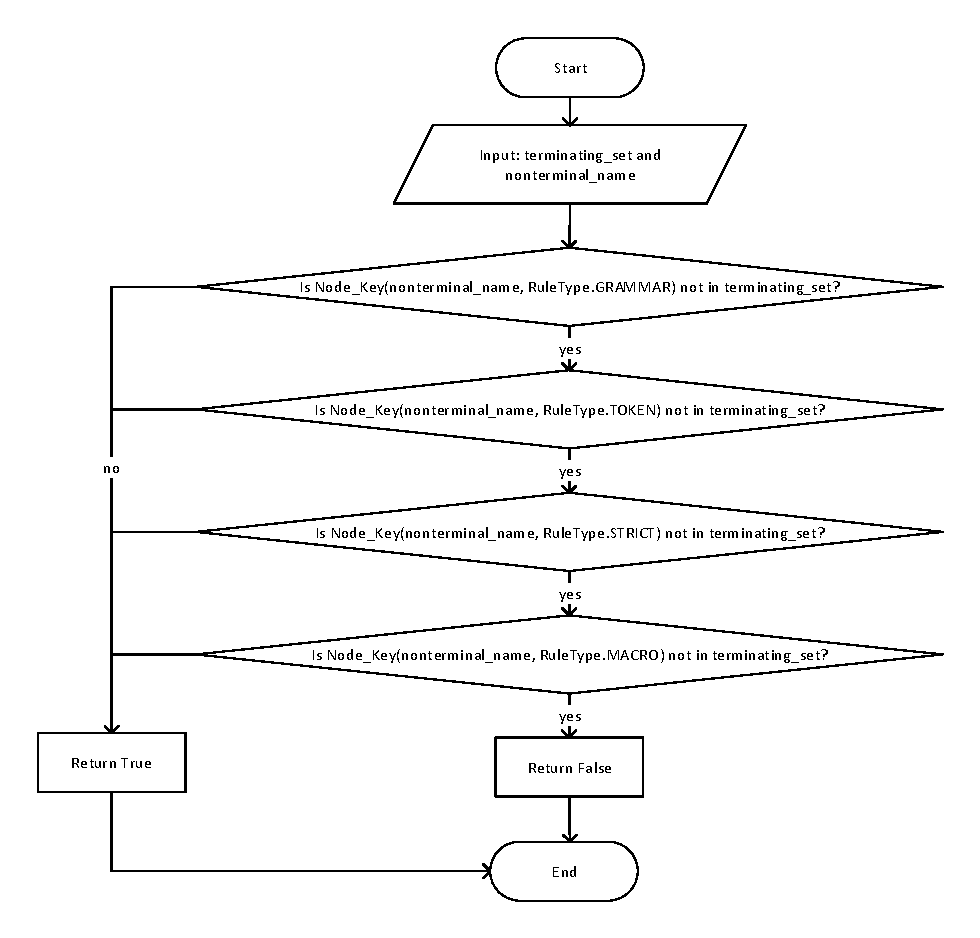
\includegraphics[width=1\textwidth]{images/Implementation_value_in_terminating.pdf}
\caption{Check if node value is in terminating set}
\label{fig:ImplementationCheckIfValueInTerminating}
\end{figure}

After the terminating symbols have been determined, productions that contain a nonterminating symbol have to be removed from the nodes of the grammar graph because some nonterminal symbols might have productions that contain nonterminating symbols, but also other productions that only contain terminating symbols. Only the productions containing nonterminating symbols have to be removed.\\
Algorithm \ref{alg:delete_non_terminating_productions}  describes how productions that include nonterminating symbols are removed from the grammar graph.
The start node of the graph, the set of known terminating nodes and an empty set of already visited nodes are input at the first call of the algorithm.
If the input node has been visited before it is not visited again, and the algorithm ends.
If it has not been visited before the corresponding \textit{Node\textunderscore Key} is added to the set of visited nodes.
Then the \textit{children} list of the node is iterated (line 5).
The index created in line 4 corresponds to the current element of the \textit{children} list, that is iterated.
It is needed to delete the \textit{children} list and the corresponding \textit{productions\textunderscore list}, if a production contains nonterminating symbols. The \textit{children} list is iterated in reverse, because, if a \textit{children} list and \textit{productions\textunderscore list} is deleted this will not effect the indexing of the next \textit{children} list to analyse.
The \textit{children} list contains lists of nodes for each production (see section \ref{sec:sec:ConceptGraphGeneration}). Each list, nested in the \textit{children} list, is iterated and for each node the algorithm is called recursively (line 7 and 8).\\
If a node represent a nonterminating symbol the \textit{not\textunderscore terminating} flag is set to true.
If this flag is true after iteration of one element of the \textit{children} list, it means that the production corresponding to the \textit{children} list element contains at least one nonterminating symbol.
If that is the case, the corresponding element of the \textit{children} list and of the \textit{productions\textunderscore list} are removed from the node.
This is repeated for all elements of the \textit{children} list.

As a result of this algorithm, all productions that contained nonterminal symbols have been removed from the grammar graph.

\begin{algorithm}[H]
\caption{Delete non terminating productions}
\begin{algorithmic}[1] 
\Require node, terminating\textunderscore set, visited\textunderscore set
\State node\textunderscore key = Node\textunderscore Key(node.value, node.rule\textunderscore type)
\If{node\textunderscore key not in visited\textunderscore set}
	\State visited\textunderscore set.add(node\textunderscore key)
	\State index = len(node.children) - 1
	\ForAll {children\textunderscore list in reversed(node.children)}
		\State not\textunderscore terminating = False
		\ForAll {child in children\textunderscore list}
			\State delete\textunderscore non\textunderscore terminating\textunderscore productions(child, terminating\textunderscore set, visited\textunderscore set)
			\If{not value\textunderscore in\textunderscore terminating(child.value, terminating\textunderscore set)}
				\State not\textunderscore terminating = true
			\EndIf
		\EndFor
		\If{not\textunderscore terminating}
			\State delete node.children[index]
			\State delete node.productions\textunderscore list.list[index]
		\EndIf
		\State index = index - 1
\EndFor
\EndIf
\end{algorithmic}
\label{alg:delete_non_terminating_productions}
\end{algorithm}

After the productions containing nonterminating symbols have been removed from the grammar graph, the nodes that represent nonterminating symbols can also be removed from the \textit{nodes\textunderscore dictionary}.
Algorithm \ref{alg:delete_non_terminating_nodes} is responsible for this. It takes the set of \textit{Node\textunderscore Key}s as input, that specifies all terminating nodes.
To remove the nonterminating nodes, in a for-loop, all terminating nodes that are addressed by the \textit{Node\textunderscore Key}s are stored in a temporary dictionary. This dictionary replaces the original \textit{nodes\textunderscore dictionary} of the \textit{TPTPGraphBuilder}.
\begin{algorithm}[H]
\caption{Delete non terminating nodes}
\begin{algorithmic}[1] 
\Require terminating\textunderscore set
\State temporary\textunderscore dictionary = \{\}
\ForAll{node\textunderscore key in terminating\textunderscore set}
	\State value = this.nodes\textunderscore dictionary.get(node\textunderscore key, None)
	\State temporary\textunderscore dictionary.update({node\textunderscore key: value})
\EndFor
\State this.nodes\textunderscore dictionary = temporary\textunderscore dictionary
\end{algorithmic}
\label{alg:delete_non_terminating_nodes}
\end{algorithm}

\subsection{Determination of the remaining reachable symbols}

Now, that nonterminating symbols have been removed from the grammar graph, the remaining reachable symbols have to be determined.
As described in section \ref{sec:ConceptRemovingBlockedProductions} the determination of the remaining reachable is done by creating a new grammar graph, with the desired start symbol from the control file.
The new grammar graph will only contain the reachable symbols (as described in section \ref{sec:ConceptDerterminingRemainingReachable}). 

\section{Input}\label{sec:ImplementationInput}

There are two methods performing input operations that are explained in the following. 

\subsubsection{Import\textunderscore tptp\textunderscore syntax\textunderscore from\textunderscore web}

The method $import\textunderscore tptp\textunderscore syntax\textunderscore from\textunderscore web$ shown in listing \ref{
:ImplementationInputWeb} is used get a text from a website. \\
For opening a \ac{URL}, the library urllib is used. $Urllib.request$ opens a specified \ac{URL} and sends an HTTP request. $Urlopen$ returns a response object for the initiated request. The response is a file-like object that can be read using $.read()$. \cite{urllib} \\
The file can then be converted from html to text format using BeautifulSoup's html parser.
The header from the file is deleted because it does not belong to the \ac{TPTP} syntax but is appended by urllib. The header is deleted by splitting the grammar file at ever new line and joining all lines excluding the first one. \\

\begin{lstlisting}[language=Python, basicstyle=\scriptsize	,caption= Import TPTP syntax from web,label= lst:ImplementationInputWeb]
with urllib.request.urlopen("http://www.tptp.org/TPTP/SyntaxBNF.html") as url:
        html_doc = url.read()
soup = BeautifulSoup(html_doc, 'html.parser')
tptp_grammar = soup.get_text()
# Delete Header
tptp_grammar = '\n'.join(tptp_grammar.split('\n')[1:])
\end{lstlisting}

\subsubsection{Read\textunderscore text\textunderscore from\textunderscore file}

$Read\textunderscore text\textunderscore from\textunderscore file$ in listing \ref{lst:ImplementationInputText} uses the build-in function $open$ to read a text file. \\

\begin{lstlisting}[language=Python, basicstyle=\scriptsize	,caption= Read text from file,label= lst:ImplementationInputText]
with open(filename, 'r') as text_file:
        text = text_file.read()
\end{lstlisting}

\section{Output generation}\label{sec:ImplementationOutputGeneration}

- creating print list\\ 
- saving print list to file

\subsection{Create output from grammar graph}\label{sec:ImplementationOutputGrammarGraph}

For saving the grammar graph in a text file, the graph needs to be traversed and converted to a string format that can be saved to a text document. The grammar graph is converted to a string format by converting every rule to a string and coheres them. Every rule is represented by a node and the nodes children list. Therefore, the graph is traversed and string representation of the nodes are created.
The final output is stored in a $print\textunderscore list$. A $print\textunderscore list$ is a list of $print\textunderscore list\textunderscore entries$ that can be seen in listing\ref{lst:ImplementationOutputPrintListEntry}. A $print\textunderscore list\textunderscore entry$ is a string consisting of the position of the rule that is represented by the node in the original \ac{TPTP} grammar and a string version of the rule or rather the node and its children list.

\begin{lstlisting}[language=Python, basicstyle=\scriptsize	,caption= Print List Entry,label= lst:ImplementationOutputPrintListEntry]
PrintListEntry = namedtuple("PrintListEntry", ["position", "string"])
\end{lstlisting}

The detailed process of saving a grammar graph in a text file is described in the following sections.

\subsubsection{Saving string representation of graph in text file}\label{sec:ImplementationOutputSaveGrammarGraphStringRepresentations}

In order to create the $print\textunderscore string$ the $print\textunderscore list$ is generated. For generating the $print\textunderscore list$, an empty set $visited$ is created that is used for memorising which nodes have already been visited. Moreover, an empty $print\textunderscore list$ and $print\textunderscore string$ are created. The set $visited$ and the empty $print\textunderscore list$ are used for calling the function $create\textunderscore print\textunderscore list$ (see following section) which returns the final $print\textunderscore list$. Because the rules in the $print\textunderscore list$ are not in the same order as the rules in the original \ac{TPTP} syntax, the $print\textunderscore list$ is sorted based on the rule's position that is stored in the first element of the $PrintListEntry$ tuple. For converting the $print\textunderscore list$ to one string, the $print\textunderscore string$, the $print\textunderscore list$ is iterated. Except for the first element of the list, every element of the list is added to the $print\textunderscore string$. This is done by adding the strings that are stored in the second element of the $PrintListEntry$ tuple and separating them by a new line. The first element is not added because it represents the general start symbol that has been added to the grammar (see chapter \ref{sec:ConceptGraphGeneration} but is not a part of the \ac{TPTP} grammar. A text document with a filename that has been selected by the user is then opened and the $print\textunderscore string$ is written to the file.
The simplified process can be seen in the flow diagram in figure \ref{fig:ImplementationOutputSaveOrderedRules}.

\begin{figure}[H]
\centering
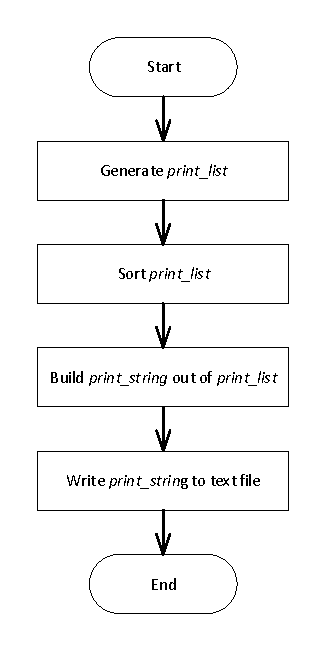
\includegraphics[width=0.4\textwidth]{images/Implementation_saveorderedrules.pdf}
\caption{Save ordered rules from graph}
\label{fig:ImplementationOutputSaveOrderedRules}
\end{figure}

\subsubsection{Traverse graph to create string representations of objects}\label{sec:ImpolementationOutputGrammarGraphTraverse}

The graph is traversed using the function $create\textunderscore print\textunderscore list$. For every node a new $print\textunderscore list\textunderscore entry$ is created. The str function that is called to create the $print\textunderscore list\textunderscore entry$ is described in section \ref{sec:ImplementationOutputGrammarGraphStringRepresentations}. 
The $print\textunderscore list\textunderscore entry$ is then appended to the $print\textunderscore list$. Once visited a node is added to the set $visited$ so that it will not be visited again.
Recursively all children in the node's children list are traversed. Because a child can once again have a list, every element of the child's list is considered and calls $create\textunderscore print\textunderscore list$ to complete the final $print\textunderscore list$. The visited elements are then also added to visited set. The algorithms ends with returning his version of the $print\textunderscore list$ that will be complete list once the first node who called the function return its $print\textunderscore list$.

\begin{algorithm}[H]
\caption{Output Algorithm: create\textunderscore print\textunderscore list}\label{alg:OutputCreatePrintList}
\begin{algorithmic}[1] 
\Require node, visited, print\textunderscore list
\State Create PrintListEntry with node.position and str(node)
\State Append PrintListEntry to print\textunderscore list
\State Add node to visited
\ForAll {children in node.children} 
	\ForAll {elements in children} 
		\If {element is not in visited}
			\State print\textunderscore list = create\textunderscore print\textunderscore list(element, visited, print\textunderscore list)
			\State Add element to visited
		\EndIf
	\EndFor
\EndFor \\
\Return print\textunderscore list
\end{algorithmic}
\end{algorithm}

\subsubsection{Create string representations of objects}\label{sec:ImplementationOutputGrammarGraphStringRepresentations}

-create str from node
-node creates str represenation of attributes internally
-following classes implement str method:
-maybe examples from syntax file

\subsubsection{\textit{NTNode} string representation creation}

-goal is to create string with comment and rule, the same way like in the original syntax

NTNODE (UML diagram in figure \ref{fig:ImplementationNTNodeUML})
-node represents rule and comment block associated with node
-consists of comment block
-rule type table ref
-whitespace padding

called here:
-create string representation of comment block
-also create string represent

\begin{algorithm}[H]
\caption{\textit{NTNode} string creation}\label{alg:OutputCreateNodeString}
\begin{algorithmic}[1] 
\If {this.comment\textunderscore block is not None}
	\State node\textunderscore string += str(this.comment\textunderscore block)
\EndIf
\State node\textunderscore string += this.value
\State add whitespace padding
\If{this.rule\textunderscore type == RuleType.GRAMMAR}
	\State node\textunderscore string += " ::= "
\ElsIf{this.rule\textunderscore type == RuleType.TOKEN}
	\State node\textunderscore string += " ::- "
\ElsIf{this.rule\textunderscore type == RuleType.STRICT}
	\State node\textunderscore string += " :== "
\ElsIf{this.rule\textunderscore type == RuleType.MACRO}
	\State node\textunderscore string += " ::: "
\EndIf
\State node\textunderscore string += str(this.productions\textunderscore list)
\Return node\textunderscore string
\end{algorithmic}
\end{algorithm}

\subsubsection{\textit{COMMENT\textunderscore BLOCK} string representation creation}

The \textit{COMMENT\textunderscore BLOCK} class has a list of comment lines as an attribute (see UML diagram in figure \ref{fig:ConceptCommentBlockClassDiagram}). The string representation of the \textit{COMMENT\textunderscore BLOCK} objects is created by concatenating the comment lines, separating them by newline characters.

\subsubsection{\textit{PRODUCTIONS\textunderscore LIST} string representation creation}

The \textit{PRODUCTIONS\textunderscore LIST} class contains a list of production alternatives of a rule (the right-hand side of a rule). The production alternatives are separated by " | " in the original \ac{TPTP} syntax.

-listing example

Algorithm \ref{alg:OutputCreateProductionsListString} shows the process of creating the string representation of a \textit{PRODUCTIONS\textunderscore LIST}. The productions in \textit{PRODUCTIONS\textunderscore LIST} are iterated and the string representation of every production is created (described in ...) and the productions are separated by the " | " string. The counter is used to identify the last production and not print alternative symbol after that production.

\begin{algorithm}[H]
\caption{\textit{PRODUCTIONS\textunderscore LIST} string creation}\label{alg:OutputCreateProductionsListString}
\begin{algorithmic}[1]
\State productions\textunderscore list\textunderscore string = ""
\State length = length(this.list)
\State counter = 1
\ForAll{production in this.list}
	\State productions\textunderscore list\textunderscore string += str (production)
	\If{counter < length}
		\State productions\textunderscore list\textunderscore string += " | "
	\EndIf
	\State index += 1
\EndFor
\State Return \State productions\textunderscore list\textunderscore string
\end{algorithmic}
\end{algorithm}

\subsubsection{\textit{PRODUCTION} string representation creation}

The \textit{PRODUCTION} class has a \textit{list} of element and a \textit{ProductionProperty} as an attribute (see UML diagram in figure \ref{fig:ConceptProductionClassDiagram}).
The elements of the list of a \textit{PRODUCTION} can be of type \textit{PRODUCTION}, \textit{PRODUCTION\textunderscore ELEMENT}, and \textit{XOR\textunderscore PRODUCTIONS\textunderscore LIST}.\\
Algorithm \ref{alg:OutputCreateProductionString} describes the procedure of creating the string representation of a \textit{PRODUCTION}.
First, the \textit{production\textunderscore string} is initialised.
Then, depending on the \textit{ProductionProperty} ?symbols? are added to the \textit{production\textunderscore string}.
If the \textit{ProductionProperty} is \textit{NONE} no special symbols need to be added.
In case of the \textit{ProductionProperty} \textit{REPETITION}, the open parenthesis character "(" is added to the \textit{production\textunderscore string} in order to enclose the \textit{list} elements.
In case of the \textit{ProductionProperty} \textit{OPTIONAL}, the elements have to be enclosed in square brackets. Therefore the "[" character is added to the \textit{production\textunderscore string} in that case.\\
After that, the \textit{list} is iterated and the string representation of each element is created and added to the \textit{production\textunderscore string}.\\
Again depending on the \textit{ProductionProperty} additional characters might have to be added.
In case of the \textit{ProductionProperty} \textit{REPETITION} the open parenthesis is closed with the close parenthesis and the repetition symbol is added to denote the repetition property.
In case of the \textit{ProductionProperty} \textit{OPTIONAL} the open square bracket is closed.
Then the created \textit{production\textunderscore string} is returned.

\begin{algorithm}[H]
\caption{\textit{PRODUCTION} string creation}
\label{alg:OutputCreateProductionString}
\begin{algorithmic}[1]
\State production\textunderscore string = ""
\If{self.productionProperty == ProductionProperty.REPETITION}
	\State production\textunderscore string += "("
\ElsIf {element.productionProperty == ProductionProperty.OPTIONAL}	
	\State production\textunderscore string += "["
\EndIf
\ForAll{element in this.list}
		\State production\textunderscore string += str(element)
\EndFor
\If{self.productionProperty == ProductionProperty.REPETITION}
	\State production\textunderscore string += ")*"
\ElsIf {element.productionProperty == ProductionProperty.OPTIONAL}	
	\State production\textunderscore string += "]"
\EndIf
\State Return production\textunderscore string
\end{algorithmic}
\end{algorithm}

\subsubsection{\textit{XOR\textunderscore PRODUCTIONS\textunderscore LIST} string representation creation}
The procedure to create the string representation of the \textit{XOR\textunderscore PRODUCTIONS\textunderscore LIST} class is equivalent to the \textit{PRODUCTIONS\textunderscore LIST} process described in algorithm \ref{alg:OutputCreateProductionsListString} with the difference that generated string is enclosed by parentheses.
\subsubsection{\textit{PRODUCTION\textunderscore ELEMENT} string representation creation}

-production element symbol with production property 

\begin{algorithm}[H]
\caption{\textit{PRODUCTION\textunderscore ELEMENT}  string creation}
\label{alg:OutputCreateProductionElementString}
\begin{algorithmic}[1]
\State production\textunderscore element\textunderscore string = ""
	\If {element.productionProperty == ProductionProperty.NONE}
		\State production\textunderscore string += str(this.symbol)
	\ElsIf {element.productionProperty == ProductionProperty.REPETITION}	
		\State production\textunderscore string += "("
		\State production\textunderscore string += str(this.symbol)
		\State production\textunderscore string += ")"
		\State production\textunderscore string += "*"
	\ElsIf {element.productionProperty == ProductionProperty.OPTIONAL}	
		\State production\textunderscore string += "["
		\State production\textunderscore string += str(this.symbol)
		\State production\textunderscore string += "]"
	\EndIf
\State production\textunderscore element\textunderscore string
\end{algorithmic}
\end{algorithm}

\subsubsection{Symbol string representation creation}

-The nonterminal symbol value can be returned as is
-nt, terminal symbol
-check t symbol str

\subsection{Automated parser generator compatibility}\label{sec:ImplementationAutomatedParserGenerator}

-append option

\section{GUI}\label{sec:ImplementationGUI}

The GUI consists of the class View that can be seen in Figure \ref{fig:ImplementationViewClassDiagram}. The class has the attributes $treeView$ which is an instance of the PyQt QTreeWidget, $graphBuilder$ which is an instance of the TPTPGraphBuilder and the boolean value $commentStatus$. The class functions and their implementation are described in the following sections based on the five sub-menus.

\begin{figure}[H]
\centering
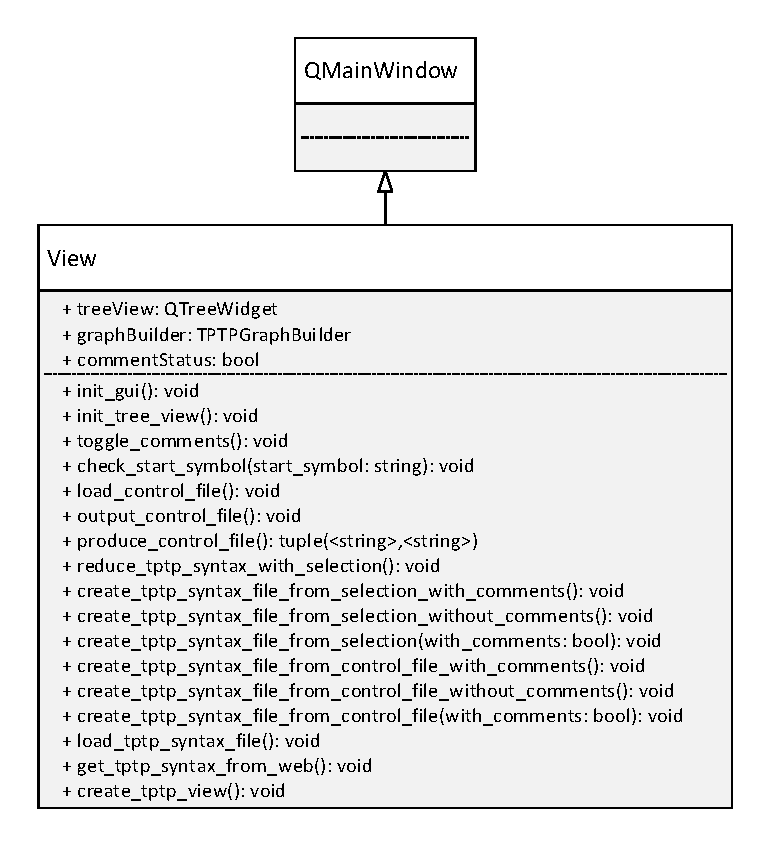
\includegraphics[width=0.8\textwidth]{images/Implementation_view_class_diagramm.pdf}
\caption{View UML class diagram}
\label{fig:ImplementationViewClassDiagram}
\end{figure}

\subsection{Main application window}\label{sec:ImplementationGUIMainAppli}

\subsubsection{Init GUI}\label{sec:ImplementationGUIInit}

The function $init\textunderscore gui$ sets up the menu bar in the main application window. The menu bar consists of the sub-menus "Import syntax", "Save syntax", "Reduce", "Control file" and "View". To each sub-menu menu actions that have been described in chapter \ref{sec:ConceptGUI} are added and implemented using QActions. The following listing \ref{lst:ImplementationInitGUI} shows the Python code for adding a menu bar and menu actions for example for the "Import syntax" menu bar.

\begin{lstlisting}[language=Python, basicstyle=\scriptsize	,caption= Implementation of menu bar,label= lst:ImplementationInitGUI]
import_menu = menubar.addMenu("Import syntax")
import_menu.addAction(import_tptp_file_action)
import_menu.addAction(import_tptp_file_from_web_action)
\end{lstlisting}

Besides a name, a short cut for executing the menu action is defined. Also, triggers have been defined that triggers functions once menu button is pressed. Listing \ref{lst:ImplementationInitGUI2} shows how a short cut and a trigger have been defined for the action $Import TPTP syntax file$.

\begin{lstlisting}[language=Python, basicstyle=\scriptsize	,caption= Implementation of menu actions,label= lst:ImplementationInitGUI2]
import_tptp_file_action = QAction('&Import TPTP syntax file', self)
import_tptp_file_action.setShortcut('Ctrl+O')
import_tptp_file_action.triggered.connect(self.load_tptp_syntax_file)
\end{lstlisting}


\subsubsection{Init TreeView}\label{sec:ImplementationGUIInitTreeView}
Init TreeView is used for displaying a grammar in the main application window. The method is called after importing or reducing a grammar. The grammar is stored in a nodes dictionary whose values (the nodes) are then converted to a list. This list is displayed by transforming it into a tree view. A tree view can be used for displaying nested lists and allowing a user to navigate through them. The tree view consists of all nodes whose leaves are the productions in their (nested) productions list. The nodes can be expanded to see their productions which are then displayed indented and underneath the node.

A new tree view is defined using QTreeWidget with the header labels "Nonterminal", "Production Type" and "Production" (line 1 and 2 in listing \ref{lst:ImplementationInitTreeView}).
All nodes of the nodes dictionary of the GraphBuilder instance are extracted and sorted based on their position in the original \ac{TPTP} syntax file (line 3 and 4 in listing \ref{lst:ImplementationInitTreeView}. 
The pseudo code in \ref{alg:initTreeView} shows the code used for filling the created treeView. For every node a new QTreeWidgetItem is generated. The item consists of the nodes (node.value) and its rule type. Also a new checkbox is defined that is displayed next to the item whose initial value is unchecked. The background colour to set to grey.
For every production in the nodes production list, a new QTreeWidgetItem and checkbox are created as well. However, the default value of the checkbox is set to unchecked. The generated item is then added as a child to the node item. A potential comment block is added to the treeView and the item is added to the treeView as well.

\begin{lstlisting}[language=Python, basicstyle=\scriptsize	,caption= Init Tree View,label= lst:ImplementationInitTreeView]
self.treeView = QTreeWidget()
self.treeView.setHeaderLabels(['Non Terminal', 'Production Type', 'Production'])
nodes_list = list(self.graphBuilder.nodes_dictionary.values())
nodes_list.sort(key=lambda x: x.position)
\end{lstlisting}

\begin{algorithm}[H]
\caption{GUI Pseudo Code: init\textunderscore tree\textunderscore view}
\label{alg:initTreeView}
\begin{algorithmic}[1] 
\ForAll {nodes in nodes\textunderscore list}
	\State rule\textunderscore type = node.rule\textunderscore type
	\State item = new QTreeWidgetItem
    \State Uncheck checkbox of item 
    \State Set background to grey
	\ForAll {productions in node.productions\textunderscore list}
		\State child\textunderscore item = new QTreeWidgetItem
		\State Check checkbox of child item
		\State Add child\textunderscore item to item
	\EndFor    
	\If {node.comment\textunderscore block exists}
		\State comment\textunderscore item = new QTreeWidgetItem
		\State Add comment\textunderscore item to treeView
	\EndIf
	\State Add item to treeView
\EndFor
\end{algorithmic}
\end{algorithm}

\subsection{Import menu}\label{sec:ImplementationGUIImportMenu}	
\subsubsection{Import \ac{TPTP} syntax file}\label{sec:ImplementationGUIImportFile}

The \ac{TPTP} syntax file is imported using QFileDialog which is returning the filename. If the filename is not empty, the application opens a dialog window where the user has to specify a desired start symbol. The method $red\textunderscore text\textunderscore from\textunderscore file$ returns the text of the file belonging to the filename. With the textfile and the start symbol, the method $create\textunderscore tptp\textunderscore view$ is called.

\subsubsection{Import \ac{TPTP} syntax from the \ac{TPTP} website}\label{sec:ImplementationGUIImportInternet}

The \ac{TPTP} syntax file is extracted from the \ac{TPTP} website using the Input method $import\textunderscore tptp\textunderscore syntax\textunderscore from\textunderscore web$ (see chapter REF). This method returns a textfile. The application opens a dialog window where the user has to specify a desired start symbol. With the textfile and the start symbol, the method $create\textunderscore tptp\textunderscore view$ is called.

$create\textunderscore tptp\textunderscore view$ \\
The method creates a new instance of the $TPTPGraphBuilder$, calls $graphBuilder.run$, $init\textunderscore tree\textunderscore view$ and $check\textunderscore start\textunderscore symbol$.

\subsubsection{Check start symbol}\label{sec:ImplementationGUIStartsymbol}

This function checks the checkbox of the defined start symbol. The QTreeView method $findItem(string\; itemName)$ is used that returns all items that match the item name. 
The found items are then checked.

\subsection{View menu}\label{sec:ImplementationGUIViewMenu}
\subsubsection{Toggle comments}\label{sec:ImplementationGUIToggleComments}

Algorithm \ref{alg:toggleComments} shows the algorithm used for toggling comments. The algorithm should either show or hide the comments based on the current state. 
The View class attribute $commentStatus$ indicates whether comments are displayed (true) or not (false). For toggling comments, a new status is set that is the opposite of $commentStatus$. While looping through every item in $treeView$, comment items can be found by checking whether the item is checkable because by default a comment is not checkable by the user. A QTreeWidgetItem has flags including a flag "ItemIsUserCheckable" that is used for determining whether the item is checkable. The QTreeWidgetItem function $setHidden(bool\;hide)$ is applied on every comment with the value of the new status. CommentStatus is set to the new status. 

-flag(), bitweises AND 

\begin{algorithm}[H]
\caption{GUI Algorithm: toggle\textunderscore comments}
\label{alg:toggleComments}
\begin{algorithmic}[1] 
\State newStatus = not commentStatus
\ForAll {items in treeView}
	\If {item is not checkable}
		\State item.setHidden(newStatus)
	\EndIf
\EndFor
\State commentStatus = newStatus
\end{algorithmic}
\end{algorithm}

\subsection{Reduce menu}\label{sec:ImplementationGUIReduceMenu}
\subsubsection{Reduce \ac{TPTP} syntax with selection}\label{sec:ImplementationGUIReduceWithSelection}

The method reduce \ac{TPTP} syntax with selection reduces the syntax and displays the resulting syntax in the GUI. 
For reducing the \ac{TPTP} syntax based on the users selection in the GUI a control file is produced (see Produce Control file). If no grammar has been imported or no start symbol or multiple start symbol have been selected an error is raised. The error is displayed using a QMessageBox. With the produced control file, the Graphbuilder disables blocked productions, treeView is initialized and the start symbol is checked (see listing \ref{lst:ImplementationGUIReduceTPTPSelection}). 

\begin{lstlisting}[language=Python, basicstyle=\scriptsize	,caption= Reduce TPTP syntax with selection,label= lst:ImplementationGUIReduceTPTPSelection]
control_string, start_symbol = self.produce_control_file()
self.graphBuilder.disable_rules(control_string)
self.init_tree_view()
self.check_start_symbol(start_symbol)
\end{lstlisting}
\subsection{Save syntax menu}\label{sec:ImplementationGUISaveSyntaxMenu}
\subsubsection{Create \ac{TPTP} syntax file from selection}\label{sec:ImplementationGUICreateTPTPFromSelection}

Figure \ref{fig:ImplementationGUIReduceandSave} shows a flow diagram of the process of reducing and saving a \ac{TPTP} syntax file from a user's selection.
The input of this method is a boolean value $with\textunderscore comments$ that describes if the syntax should be saved with or without comments for the automatic parser generator (see chapter \ref{sec:ValidationAutomatedParserGeneration}). 
First, the filename is import using a $QFileDialog$.
If the import is successful, meaning a filename has been selected, a control file based on user's selection is produced. If the import is not successful, the method terminates. \\
In comparison to \textit{Reduce \ac{TPTP} syntax with selection} the reduced syntax is not displayed in the GUI but only saved to local storage and the GUI displays still the full syntax. If the user wishes to display the reduced syntax in the GUI and save it, he can use the button \textit{Reduce \ac{TPTP} syntax with selection} and then use the button \textit{Reduce and save \ac{TPTP} syntax with selection}.
Because the full syntax is still displayed, the graphBuilder object storing the syntax cannot be modified. Therefore, the old graphBuilder is copied to a new graphBuilder object. Because the old object should not change, the new object should have copies of all objects that are part of the graphBuilder rather than references.
To copy the graphBuilder object which is a compound object it is necessary to use $copy.deepcopy$ instead of $copy.copy$. Deepcopy creates a new object and inserts copies of all objects that are part of to be copied object. Copy however, creates a new object and inserts references to the to be copied objects. 
The new graphBuilder is initialized with the start symbol that has been provided by the generated control file and rules that include blocked productions are disabled. During the initialization the new start symbol $<start\textunderscore symbol>$ has been added (see chapter \ref{sec:ConceptGraphGeneration} for explanation).
This start symbol is searched in the reduced syntax.
If it can be found, the syntax is saved with or without comments based on the input parameter.
However, if the start symbol cannot be found in the syntax no part of the grammar is terminating.
In this case the saved file is empty.
To save the grammar the method $Output.save\textunderscore ordered\textunderscore rules\textunderscore from\textunderscore graph(\textunderscore with\textunderscore comments)$ is used.

\begin{figure}[H]
%\centering
\includegraphics[width=1.05\textwidth]{images/implementation_reduce_and_save_tptp_syntax.pdf}
\caption{Reduce and save \ac{TPTP} syntax}
\label{fig:ImplementationGUIReduceandSave}
\end{figure}

Each button in the sub-menu has an associated action.
This action is triggered once the button is pressed. In the GUI there are two options of reducing and saving the \ac{TPTP} syntax namely \textit{Reduce and save \ac{TPTP} syntax with selection} and \textit{Reduce and save \ac{TPTP} syntax from selection with external comments}.
These two options both call the function described above and in figure \ref{fig:ImplementationGUIReduceandSave}. However, one calls it and passes $with\textunderscore comments$ as true and the other as false.
Because each button in the GUI needs it own designated function to call, the functions $create\textunderscore tptp\textunderscore syntax file\textunderscore from\textunderscore selection\textunderscore with\textunderscore comments$ and $create\textunderscore tptp\textunderscore syntax file\textunderscore from\textunderscore selection\textunderscore without\textunderscore comments$ are introduced.
They simply set the parameter $with\textunderscore comments$ accordingly and call the function \textit{Create \ac{TPTP} syntax file from selection}.

\subsubsection{Create \ac{TPTP} syntax file from control file}\label{sec:ImplementationGUICreateTPTPFromControlfile}

The previous section explained how a \ac{TPTP} syntax is reduced and saved based on a user's selection in the GUI.
The described function in this section also reduces and saves a \ac{TPTP} syntax but this time based on an imported control file.
The function is similar to the previous function \textit{Create \ac{TPTP} syntax file from selection}.
Figure \ref{fig:ImplementationGUIReduceandSaveControl} shows the same flow diagram as figure \ref{fig:ImplementationGUIReduceandSave} but highlights applied changes in red.
Changes are that besides importing a filename, a name for the control file has to be imported as well.
Instead of producing a control file based on the users selection, the specified control file is read and the grammar graph is initialised with the start symbol that is specified in the first line of the control file.

Also similar to the previous section, the functions \\ $create\textunderscore tptp\textunderscore syntax\textunderscore from\textunderscore control\textunderscore file\textunderscore with\textunderscore comments$ and \\
$create\textunderscore tptp\textunderscore syntax\textunderscore from\textunderscore control\textunderscore file\textunderscore without\textunderscore comments$ are introduced that set the parameter $with\textunderscore comments$ accordingly and call the function \textit{Create \ac{TPTP} syntax file from control file}.

\begin{figure}[H]
%\centering
\includegraphics[width=1.05\textwidth]{images/implementation_reduce_and_save_tptp_syntax_control.pdf}
\caption{Reduce and save \ac{TPTP} syntax from control file}
\label{fig:ImplementationGUIReduceandSaveControl}
\end{figure}

\subsection{Control file menu}\label{sec:ImplementationGUIControlFileMenu}
\subsubsection{Import control file}\label{sec:ImplementationGUIImportControlFile}

If a control file is imported, checkboxes have to be set accordingly. The pseudo code in \ref{alg:importControlfile} shows the process. 
The name of the control file is read in using a QFileDialog. The file itself is imported using the method $Input.read\textunderscore text\textunderscore from\textunderscore file$ (see chapter REF). If the file exists and if a tree view exists thus a grammar has been imported, all nodes are unchecked and all leaves/productions are checked. The items can be distinguished by looking for whether an item has parents and if not if it is checkable. The checkboxes are set this way because the default mode is that all nodes are unchecked and all productions are checked.  
After setting the checkboxes to the default mode, the first line of the control string is read and the start symbol is set accordingly. If there are multiple start symbols, every start symbol is checked.
Iterating every line of the control string, the nt\textunderscore name which is the first element of a line is saved and the rule\textunderscore type which is the second element as well. The item that belongs to nt\textunderscore name is then searched and every production whose index is listed in the control file is unchecked.

\begin{algorithm}[H]
\caption{GUI Pseudo Code: load\textunderscore controlfile}
\label{alg:importControlfile}
\begin{algorithmic}[1] 
\State Import Control File
\If {Control File exists}
\ForAll {items in tree view}
	\If {parent of item is None}
		\If {item is not a comment}
			\State Uncheck item
		\EndIf
	\Else
		\State Check item 
	\EndIf
\EndFor
\State Get first line of control file
\State Search item that represents start symbol 
\State Check item
\ForAll {lines in control file}
	\State Split line by comma
	\State nt\textunderscore name = first element of split
	\State rule\textunderscore type = second element of split
	\State Search nt\textunderscore name node in tree view
	\If{ parent is None and rule\textunderscore type matches rule\textunderscore type}
		\ForAll {indices in line}
			\If {child exists}
				\State Uncheck child
			\EndIf
		\EndFor
	\EndIf 
\EndFor
\EndIf
\end{algorithmic}
\end{algorithm} 

\subsubsection{Produce control file}\label{sec:ImplementationGUIProduceControlFile}

Algorithm \ref{alg:produceControlfile} shows how the control file used for reducing the \ac{TPTP} syntax is produced.
The index of productions that have been blocked by the user in the GUI are identified and stored in a dictionary until further processing.
The key of the dictionary is a tuple made of a value and a rule type that has to be defined alongside the dictionary.
Besides the blocked productions, the start symbol is featured in the control file as well, therefore an empty list for listing possibly multiple start symbols is created.
Multiple start symbols can occur when the nonterminal symbol has multiple rule types or if the users makes an invalid input. The dictionary is used for collecting all blocked productions. Looping through every node of the tree view it is checked, if the item has parents and its checkbox is unchecked. If so, the rule type of the parent is identified and a new tuple is defined. The index of the production in the parent's productions list is identified as well. If the tuple is not already in the dictionary, a new dictionary entry is created with the tuple as key and the index of the item as value. If the tuple is already in the dictionary, the index of the item is added to the existing indices. \\
However, if the item is checked and has no parents, the name of the item is appended to the list of start symbols. \\
If there are multiple start symbols in the list that do not have the same nonterminal value or no start symbol at all, the user made an invalid input and an error is raised. 
The final control string is made up of first entry of the start symbol list. The first entry is sufficient because the control file only specifies the start symbols name and not the rule type.
If there are multiple start symbols, they have the same nonterminal name. 
Each in a new line, the nonterminal symbol name, rule type and indices of blocked productions are appended to the control string. Within the line, the name, rule type and indices are separated by a comma.
Moreover, an error is risen if there is no imported grammar, for example the user presses the Reduce grammar button in the GUI without importing a grammar.

\begin{algorithm}[H]
\caption{GUI Algorithm: produce\textunderscore controlfile}
\label{alg:produceControlfile}
\begin{algorithmic}[1] 
\State Define new tuple Entry("Entry", ["value", "rule\textunderscore type"])
\State Create empty dictionary
\State Create empty list $start\textunderscore symbol$
\ForAll {items in treeView}
	\State Get parent of item
	\If {item has parent and is unchecked}
		\State Get rule type of parent
		\State Create entry tuple with name of parent and its rule type
		\State Get index of child from parent
		\If{entry tuple is not in dictionary}
			\State Create new dictionary entry with entry tuple as key and list containing the index of the child as value
		\Else
			\State Append index of child to list
		\EndIf
	\ElsIf {item has no parent and is checked}
		\State Append item name to start symbol list
	\EndIf
\EndFor
\State control\textunderscore string = first entry of start symbol list
\State Append all entries of dictionary to control\textunderscore string
\end{algorithmic}
\end{algorithm} 

\subsubsection{Output control file}\label{sec:ImplementationGUIOutput control file}

Output control file saves a control file to local storage. 
First, a control file is produced based using the method \textit{Produce control file}. A filename under which the control file is stored is input using a QFileDialog window. The control file is then stored using $Output.save\textunderscore text\textunderscore to\textunderscore file$.

\subsection{Exception handling}\label{sec:ImplementationGUIExceptionHandling}

Exceptions are used to handle wrong input from the user. There are three exceptions that are raised whenever the user makes a wrong input: 

\begin{itemize}
\item Multiple start symbols
\item No start symbol
\item No imported grammar
\end{itemize}

The exception \textit{multiple start symbols} is raised if the user selects multiple start symbols in the GUI and presses any Reduce button. On the contrary the exception \textit{no start symbol} is raised if the user selects no start symbol in the GUI and presses any Reduce button. The exception \textit{no imported grammar} is raised if the user starts the application and does not import a grammar but presses a button that requires a grammar for example in the Reduce, View or Control File menu.

\section{Command-line interface}\label{sec:ImplementationCommandLineInterface}

With the argparse module a command-line parser object can be created and parameters can be added to that object following the concept describet.
In the first line of listing \ref{lst:ImplementationArgparseParserConfiguration} the command-line parser object is created with a description.
Lines two to five contain the specification of the accepted arguments.
In addition to the name and short form of the name, the type, a help message, and whether the parameter is optional or not can be specified.
Default values for arguments can also be specified.
If no default value is specified and if the argument is not passed it will have the value \textit{None}.
The $action = 'store_true'$ in line 5 means, that if this argument flag is present in the command-line call, the value of this argument will be set to $True$.
If the flag is not present it's value will be set to $False$.
Argparse automatically checks the given conditions, for example if a required argument is not given and displays an error message if that is the case.

\begin{lstlisting}[language=Python, basicstyle=\scriptsize	,caption= Argparse command-line parser configuration,label= lst:ImplementationArgparseParserConfiguration]
self.argument_parser = argparse.ArgumentParser(description='Extract sub-syntax using TPTP syntax file and a control file')
self.argument_parser.add_argument('-g', '--grammar', metavar='', type=str, required=True, help='path of the TPTP syntax file')
self.argument_parser.add_argument('-c', '--control', metavar='', type=str, required=True, help='path of the control file')
self.argument_parser.add_argument('-o', '--output', metavar='', type=str, required=False, help='optional output file name (default output.txt)', default= "output.txt")
self.argument_parser.add_argument('-ec',  '--external_comment', action='store_true', help="flag - include external comment syntax")
\end{lstlisting}

Argparse will also automatically create the help output by using the descriptions provided when configuring the argument parser.
